% 98-57(98쪽) — 원에 내접하는 사각형 ABCD($\seg{AB}=3$ · $\seg{BC}=3$ · $\seg{CD}=2$ · $\seg{AD}=4$). 스캔 화질이 낮아 TikZ 로 다시 그림.
% 라벨은 원문 것만: 꼭짓점 A·B·C·D 와 길이 4·2·3·3. 각·넓이(답)는 적지 않는다.
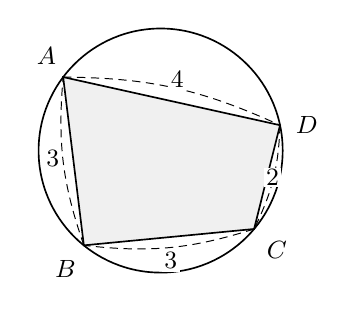
\begin{tikzpicture}[line width=0.6pt, x=1cm, y=1cm]
  \coordinate (A) at (-1.238,0.933);
  \coordinate (B) at (-0.975,-1.204);
  \coordinate (C) at (1.187,-0.996);
  \coordinate (D) at (1.516,0.322);
  \fill[black!6] (A) -- (B) -- (C) -- (D) -- cycle;
  \draw (0,0) circle (1.55);
  \draw (A) -- (B) -- (C) -- (D) -- cycle;
  % 길이 표시의 점선 호
  \draw[densely dashed, line width=0.35pt] (A) to[bend left=12] (D);
  \draw[densely dashed, line width=0.35pt] (D) to[bend left=12] (C);
  \draw[densely dashed, line width=0.35pt] (C) to[bend left=12] (B);
  \draw[densely dashed, line width=0.35pt] (B) to[bend left=12] (A);
  \node[font=\small, fill=white, inner sep=1pt] at (0.21,0.90) {$4$};
  \node[font=\small, fill=white, inner sep=0.6pt] at (1.42,-0.34) {$2$};
  \node[font=\small, fill=white, inner sep=1pt] at (0.13,-1.40) {$3$};
  \node[font=\small, fill=white, inner sep=0.6pt] at (-1.37,-0.10) {$3$};
  \node[font=\small, anchor=south east] at (-1.20,0.97) {$\pt{A}$};
  \node[font=\small, anchor=north east] at (-0.95,-1.27) {$\pt{B}$};
  \node[font=\small, anchor=north west] at (1.22,-1.03) {$\pt{C}$};
  \node[font=\small, anchor=west] at (1.59,0.32) {$\pt{D}$};
\end{tikzpicture}
